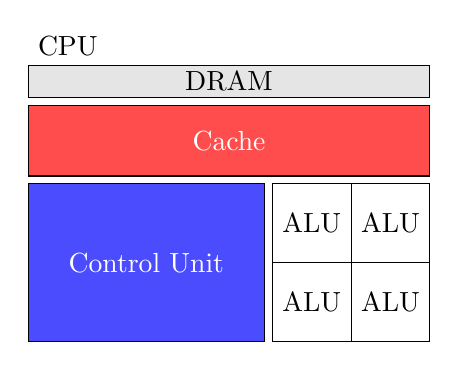
\begin{tikzpicture}
% ALUs
\foreach \x in {3,...,4}
	\foreach \y in {0,...,1}
		\draw[] (\x+.1,\y) rectangle (\x+1.1,\y+1) node[pos=.5] {ALU};
% Control Unit
\draw[fill=blue!70] (0,0) rectangle (3,2) node[pos=.5,text=white] {Control Unit};
%Cache
\draw[fill=red!70] (0,2.1) rectangle (5.1,3) node[pos=.5,text=white] {Cache};
% DRAM
\draw[fill=black!10] (0,3.1) rectangle (5.1,3.5) node[pos=.5] {DRAM};
%Name 
\node[yshift=7pt,anchor=west] at (0,3.5) {CPU};
\end{tikzpicture}
\hspace{1cm}
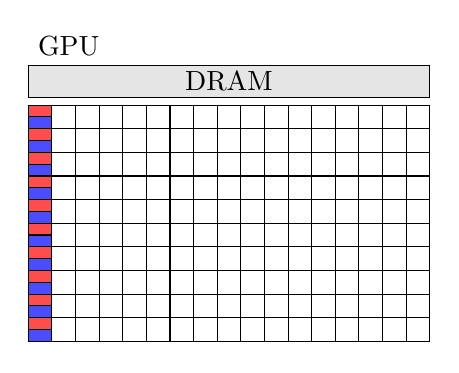
\begin{tikzpicture}
% ALUs
\foreach \y in {0,...,9}
{
	\draw[fill=blue!70] (0,\y * .3) rectangle (.3,\y * .3 + .15) node[pos=.5] {};
	\draw[fill=red!70] (0,\y * .3 + .15) rectangle (.3,\y * .3 + .3) node[pos=.5] {};
	\foreach \x in {1,...,16}
		\draw[] (\x*.3,\y*.3) rectangle (\x *.3+.3,\y*.3+.3) node[pos=.5] {};
}
% DRAM
\draw[fill=black!10] (0,3.1) rectangle (5.1,3.5) node[pos=.5] {DRAM};
% Name 
\node[yshift=7pt,anchor=west] at (0,3.5) {GPU};
\end{tikzpicture}